\apendice{Especificación de Requisitos}


\section{Diagrama de casos de uso}

En la Figura \ref{fig:cu} podemos observar el diagrama de casos de uso elaborado para este proyecto. En primer lugar, se ha identificado a los actores. En este caso el único actor sería la persona encargada de desarrollar el proyecto. Después, se identifican los diferentes casos de uso. En este diagrama contamos con 7 casos de uso diferentes:

\begin{enumerate}
    \item \textbf{CU-1} Montaje del circuito electrónico. Tabla \ref{tab:cu1}
    \item \textbf{CU-2} Llenado de tanques y colocación de mangueras.Tabla \ref{tab:cu2}
    \item \textbf{CU-3} Conexión de la placa de Arduino al ordenador. Tabla \ref{tab:cu3}
    \item \textbf{CU-4} Descargar la aplicación Arduino IDE. Tabla \ref{tab:cu4}
    \item \textbf{CU-5} Ejecución del programa. Tabla \ref{tab:cu5}
    \item \textbf{CU-6} Completar los datos. Tabla \ref{tab:cu6}
    \item \textbf{CU-7} Generar datos. Tabla \ref{tab:cu7}
\end{enumerate}
\begin{figure}[h]
    \centering
    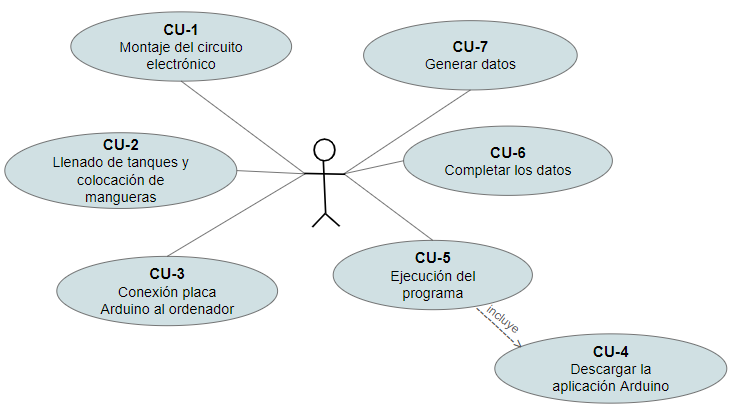
\includegraphics[width=1.2\textwidth]{img/CU.PNG}
    \caption{Diagrama de casos de uso. Imagen Propia}
    \label{fig:cu}
\end{figure}



\section{Explicación casos de uso.}

A continuación se explicarán los casos de uso mediante las tablas \ref{tab:cu1}, \ref{tab:cu2}, \ref{tab:cu3}, \ref{tab:cu4}, \ref{tab:cu5}, \ref{tab:cu6} y \ref{tab:cu7}.


% Caso de Uso 1 -> Montaje del circuito electrónico
\begin{table}[H]
	\centering
	\begin{tabularx}{\linewidth}{ p{0.21\columnwidth} p{0.71\columnwidth} }
		\toprule
            \rowcolor[HTML]{B0E0E6} 
		  \textbf{CU-1}    & \textbf{Montaje del circuito electrónico}\\
		\toprule
		\textbf{Versión}              & 1.0    \\
		\textbf{Autor}                & Celia Valladolid Portal \\
		\textbf{Descripción}          & El montaje del circuito electrónico se hará siguiendo las indicaciones recogidas en el \textit{Anexo B}. En la sección de \textit{Instalación / Puesta en marcha} podemos encontrar las instrucciones que hay que seguir para conectar todos los componentes a Arduino. \\
		\textbf{Precondición}         & Poseer todos los componentes necesarios. \\
		\textbf{Acciones}             &
		\begin{enumerate}
			\def\labelenumi{\arabic{enumi}.}
			\tightlist
                \item Conectar la placa de Arduino con la placa de pruebas.
			\item Conectar el sensor.
			\item Conectar el relé.
                \item Conectar la mini bomba y la batería.
		\end{enumerate}\\
		%\textbf{Postcondición}        & Postcondiciones (podría haber más de una) \\
		%\textbf{Excepciones}          & Excepciones \\
		\textbf{Importancia}          & Alta  \\
		\bottomrule
	\end{tabularx}
	\caption{\textbf{CU-1} Montaje del circuito electrónico.}
        \label{tab:cu1}
\end{table}

% Caso de Uso 2 -> Llenado de tanques y colocación de mangueras
\begin{table}[H]
	\centering
	\begin{tabularx}{\linewidth}{ p{0.21\columnwidth} p{0.71\columnwidth} }
		\toprule
            \rowcolor[HTML]{B0E0E6}
		\textbf{CU-2}    & \textbf{Llenado de tanques y colocación de mangueras}\\
		\toprule
		\textbf{Versión}              & 1.0    \\
		\textbf{Autor}                & Celia Valladolid Portal \\
		\textbf{Descripción}          & Colocar las mangueras en el sensor y en la mini bomba. En el caso del sensor es debido a que este no es sumergible y en el caso de la mini bomba para hacer pasar el agua. \\
		\textbf{Precondición}         & Tener montado el circuito. \\
		\textbf{Acciones}             &
		\begin{enumerate}
			\def\labelenumi{\arabic{enumi}.}
			\tightlist
                \item Colocar la manguera en uno de los puertos del sensor que haga de colchón de aire.
			\item Colocar otra manguera en la mini bomba.
                \item Llenar dos recipientes con agua, uno para el sensor y otro para la mini bomba.
		\end{enumerate}\\
		\textbf{CU relacionados}        & CU-1 \\
		%\textbf{Excepciones}          & Excepciones \\
		\textbf{Importancia}          & Alta  \\
		\bottomrule
	\end{tabularx}
	\caption{\textbf{CU-2} Llenado de tanques y colocación de mangueras.}
        \label{tab:cu2}
\end{table}

% Caso de Uso 3 -> Conexión del circuito al ordenador
\begin{table}[H]
	\centering
	\begin{tabularx}{\linewidth}{ p{0.21\columnwidth} p{0.71\columnwidth} }
		\toprule
            \rowcolor[HTML]{B0E0E6}
		\textbf{CU-3}    & \textbf{Conexión de la placa de Arduino al ordenador}\\
		\toprule
		\textbf{Versión}              & 1.0    \\
		\textbf{Autor}                & Celia Valladolid Portal \\
		\textbf{Descripción}          & Conectar la placa de Arduino al ordenador mediante el cable USB. \\
		\textbf{Precondición}         & Tener montado el circuito. \\
		\textbf{Acciones}             & Conectar el extremo USB del cable al ordenador y el otro a la placa de Arduino. \\
		\textbf{CU relacionados}        & CU-1, CU-2 \\
		%\textbf{Excepciones}          & Excepciones \\
		\textbf{Importancia}          & Alta  \\
		\bottomrule
	\end{tabularx}
	\caption{\textbf{CU-3} Conexión de la placa de Arduino al ordenador.}
        \label{tab:cu3}
\end{table}

% Caso de Uso 4 -> Descargar la app Arduino
\begin{table}[H]
	\centering
	\begin{tabularx}{\linewidth}{ p{0.21\columnwidth} p{0.71\columnwidth} }
		\toprule
            \rowcolor[HTML]{B0E0E6}
		\textbf{CU-4}    & \textbf{Descargar la aplicación Arduino IDE}\\
		\toprule
		\textbf{Versión}              & 1.0    \\
		\textbf{Autor}                & Celia Valladolid Portal \\
		\textbf{Descripción}          & Descargar la aplicación de Arduino IDE en el ordenador. Instrucciones en el \textit{Anexo B, Requisitos software}. \\
		\textbf{Precondición}         & Tener un ordenador. \\
		\textbf{Acciones}             & En el \textit{Anexo B} tenemos el enlace para descargar la aplicación. \\
		%\textbf{Excepciones}          & Excepciones \\
		\textbf{Importancia}          & Alta  \\
		\bottomrule
	\end{tabularx}
	\caption{\textbf{CU-4} Descargar la aplicación Arduino.}
        \label{tab:cu4}
\end{table}

% Caso de Uso 5 -> Cargar el programa 
\begin{table}[H]
	\centering
	\begin{tabularx}{\linewidth}{ p{0.21\columnwidth} p{0.71\columnwidth} }
		\toprule
            \rowcolor[HTML]{B0E0E6}
		\textbf{CU-5}    & \textbf{Ejecución del programa}\\
		\toprule
		\textbf{Versión}              & 1.0    \\
		\textbf{Autor}                & Celia Valladolid Portal \\
		\textbf{Descripción}          & Ejecutar el programa en la aplicación de Arduino.  \\
		\textbf{Precondición}         & Tener descargada la aplicación. \\
		\textbf{Acciones}             &
		\begin{enumerate}
			\def\labelenumi{\arabic{enumi}.}
			\tightlist
                \item Abrir la aplicación.
			\item Abrir el archivo \textit{code-sensor.ino} que podemos encontrar en la Carpeta arduino del Repositorio.
			\item Verificar y subir el código (Figura \ref{fig:verificar}).
		\end{enumerate}\\
		\textbf{CU relacionados}        & CU-1, CU-2, CU-3, CU-4 \\
		%\textbf{Excepciones}          & Excepciones \\
		\textbf{Importancia}          & Alta  \\
		\bottomrule
	\end{tabularx}
	\caption{\textbf{CU-5} Ejecución del programa.}
        \label{tab:cu5}
\end{table}

% Caso de Uso 6 -> Completar los datos
\begin{table}[H]
	\centering
	\begin{tabularx}{\linewidth}{ p{0.21\columnwidth} p{0.71\columnwidth} }
		\toprule
            \rowcolor[HTML]{B0E0E6}
		\textbf{CU-6}    & \textbf{Completar los datos}\\
		\toprule
		\textbf{Versión}              & 1.0    \\
		\textbf{Autor}                & Celia Valladolid Portal \\
		\textbf{Descripción}          & Completar los datos solicitados por el programa rellenando los campos de forma adecuada.  \\
		\textbf{Precondición}         & Haber ejecutado el programa. \\
		\textbf{Acciones}             &
		\begin{enumerate}
			\def\labelenumi{\arabic{enumi}.}
			\tightlist
                \item Abrir el monitor, paso 3 Figura \ref{fig:verificar}.
			\item Introducir nombre completo.
			\item Introducir año de nacimiento.
                \item Introducir usuario.
                \item Introducir contraseña.
		\end{enumerate}\\
		\textbf{CU relacionados}        & CU-1, CU-2, CU-3, CU-4 \\
		\textbf{Observaciones}          & Algunos campos como el año de nacimiento, usuario y contraseña, presentan restricciones. Consultar \textit{Anexo D}. \\
		\textbf{Importancia}          & Alta  \\
		\bottomrule
	\end{tabularx}
	\caption{\textbf{CU-6} Completar los datos.}
        \label{tab:cu6}
\end{table}

% Caso de Uso 7 -> Generar datos
\begin{table}[H]
	\centering
	\begin{tabularx}{\linewidth}{ p{0.21\columnwidth} p{0.71\columnwidth} }
		\toprule
            \rowcolor[HTML]{B0E0E6}
		\textbf{CU-7}    & \textbf{Generar datos}\\
		\toprule
		\textbf{Versión}              & 1.0    \\
		\textbf{Autor}                & Celia Valladolid Portal \\
		\textbf{Descripción}          & Tras haber completado correctamente los datos solicitados, el sensor empieza a realizar lecturas, identificando los cambios de presión para que la mini bomba se active al detectar un aumento dejando pasar el agua.  \\
		\textbf{Precondición}         & Haber rellenado los datos. \\
		\textbf{Acciones}             & Generar cambios de presión en el tanque donde está el sensor, para que los detecte y la mini bomba se encienda. \\
		\textbf{CU relacionados}        & CU-1, CU-2, CU-3, CU-4, CU-5 \\
		%\textbf{Excepciones}          & Excepciones \\
		\textbf{Importancia}          & Alta  \\
		\bottomrule
	\end{tabularx}
	\caption{\textbf{CU-7} Generar datos.}
        \label{tab:cu7}
\end{table}
\newpage


\section{Prototipos de interfaz o interacción con el proyecto}
Para este proyecto no se ha llegado a desarrollar una aplicación móvil que monitorice al paciente, se ha planteado como una mejora futura. No obstante, se han elaborado prototipos de la interfaz de la aplicación. En la Figura \ref{fig:inise} podemos observar la pantalla de inicio de sesión, la Figura \ref{fig:regis} se corresponde con el registro del usuario, la pantalla inicial una vez dentro de la aplicación la podemos ver en la Figura \ref{fig:appini} y por último la Figura \ref{fig:appalerta} refleja la notificación de alerta de un paciente que está sufriendo un aumento de la presión intracraneal en ese momento.

\begin{figure}[H]
    \centering
    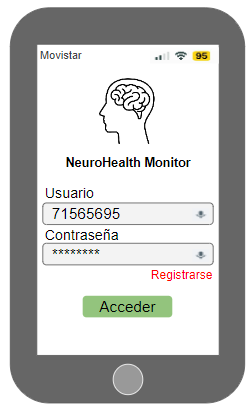
\includegraphics[width=0.4\textwidth]{img/appinicio.PNG}
    \caption{Prototipo interfaz: Inicio de sesión. Imagen propia}
    \label{fig:inise}
\end{figure}

\begin{figure}[h]
    \centering
    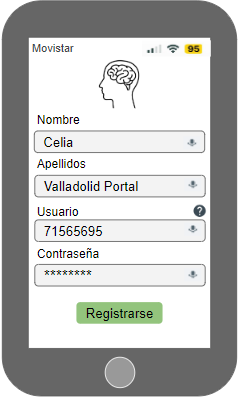
\includegraphics[width=0.4\textwidth]{img/registroapp.PNG}
    \caption{Prototipo interfaz: Registro. Imagen propia}
    \label{fig:regis}
\end{figure}

\begin{figure}[h]
    \centering
    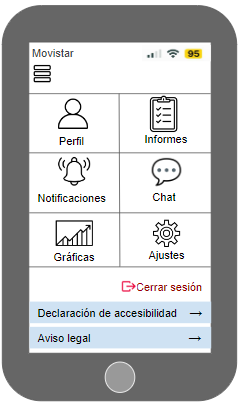
\includegraphics[width=0.4\textwidth]{img/pantallainicioapp.PNG}
    \caption{Prototipo interfaz: Pantalla inicial. Imagen propia}
    \label{fig:appini}
\end{figure}

\begin{figure}[h]
    \centering
    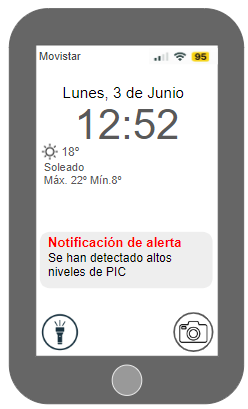
\includegraphics[width=0.4\textwidth]{img/appbloqueo.PNG}
    \caption{Prototipo interfaz: Notificación de alerta. Imagen propia}
    \label{fig:appalerta}
\end{figure}